\chapter{The SEXTANTE command--line interface}
\section{Introduction}

The command--line interface allows advanced users to increase their productivity and performe complex operations that cannot be performed using any of the other elements of the SEXTANTE GUI. Models involving several algorithms can be defined using the command--line interface, and additional operations such as loops and conditional sentences can be added to create more flexible and powerful workflows.


\section{The interface}

Invoking the command--line interface will cause the following dialog to appear.

\begin{center}
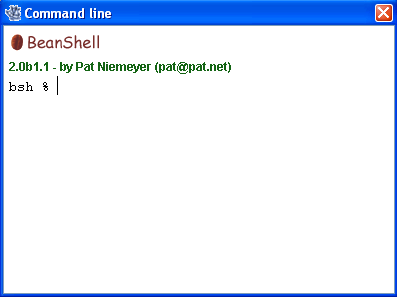
\includegraphics[width=.6\columnwidth]{command_line.png}
\end{center}

The SEXTANTE command--line interface is based on BeanShell. BeanShell is a Java source interpreter with object scripting language features, that meaning that it dynamically executes standard Java syntax and extends it with common scripting conveniences such as loose types, commands, and method closures like those in Perl and JavaScript. 

A detailed description of BeanShell and its usage can be found at the BeanShell website\footnote{\url{www.beanshell.org}}. Refer to it if you want to learn more about generic BeanShell features. This chapter covers only those particular elements which are related to SEXTANTE geoalgorithms.

By using the extension mechanisms of BeanShell, SEXTANTE adds several new commands to it, so you can run geoalgorithms or get information about the geospatial data you are using, among other things.

Java users can create small scripts and programs combining standard elements of Java with SEXTANTE commands. However, those who are not familiar with Java can also use the command--line interface to execute single processes or small sets of them, simply calling the corresponding methods.

A detailed description of all SEXTANTE commands is given next.

\subsection{Getting information about data}

Algorithms need data to run. Layers and tables are identified using the name they have in the table of contents of the GIS (and which usually can be modified using GIS tool). To call a geoalgorithm you have to pass it an identifier which represents the data to use for an input.

The \texttt{data()} command prints a list of all data objects available to be used, along with the particular name of each one (i.e. the one you have to use to refer to it). Calling it you will get something like this:

\begin{verbatim}
RASTER LAYERS
-----------------
mdt25.asc

VECTOR LAYERS
-----------------
Contour lines

TABLES
-----------------
\end{verbatim}

Be aware that some GIS allow you two have several layers with the same name. SEXTANTE will just take the first one which matches the specified identifier, so you should make sure you rename your data object so each one of them has a unique name.

To get more information about a particular data object, use the \texttt{describe(name\_of\_data\_object)} command. Here are a few examples of the result you will get when using it to get more information about a vector layer, a raster layer and a table.

\begin{verbatim}
>describe("points")
Type: Vector layer - Point
Number of entities: 300
Table fields: | ID | X | Y | SAND | SILT | CLAY | SOILTYPE | EXTRAPOLAT |

>describe("dem25")
Type: Raster layer 
X min: 262846.525725
X max: 277871.525725
Y min: 4454025.0
Y max: 4464275.0
Cellsize X: 25.0
Cellsize Y: 0.0
Rows: 410
Cols: 601

>describe("spatialCorrelation")
Type: TableNumber of records: 156
Table fields: | Distance | I_Moran | c_Geary | Semivariance | 
\end{verbatim}


\section{Getting information about algorithms}

Once you know which data you have, it is time to know which algorithms are available and how to use them. 

When you execute an algorithm using the toolbox, you use a parameters window with several fields, each one of them corresponding to a single parameter. When you use the command line interface, you must know which parameters are needed, so as to pass the right values to use to the method that runs that algorithm. Of course you do not have to memorize the requirements of all the algorithms, since SEXTANTE has a method to describe an algorithm in detail. But before we see that method, let's have a look at another one, the \texttt{algs()} method. It has no parameters, and it just prints a list of all the available algorithms. Here is a little part of that list as you will see it in your command--line shell.

\begin{verbatim}
bsh % algs();
acccost-------------------------------: Accumulated cost(isotropic)
acccostanisotropic--------------------: Accumulated cost (anisotropic)
acccostcombined-----------------------: Accumulated cost (combined)
accflow-------------------------------: Flow accumulation
acv-----------------------------------: Anisotropic coefficient of variation
addeventtheme-------------------------: Points layer from table
aggregate-----------------------------: Aggregate
aggregationindex----------------------: Aggregation index
ahp-----------------------------------: Analytical Hierarchy Process (AHP)
aspect--------------------------------: Aspect
buffer--------------------------------: Buffer
\end{verbatim}


On the right you find the name of the algorithm in the current language, which is the same name that identifies the algorithm in the toolbox. However, this name is not constant, since it depends on the current language, and thus cannot be used to call the algorithm. Instead, a command--line is needed. On the left side of the list you will find the command--line name of each algorithm. This is the one you have to use to make a reference to the algorithm you want to use.

Now, let's see how to get a list of the parameters that an algorithms require and the outputs that it will generate. To do it, you can use the \texttt{describealg(name\_of\_the\_algorithm)} method. Use the command--line name of the algorithm, not the full descriptive name.

For example, if we want to calculate a flow accumulation layer from a DEM, we will need to execute the corresponding module, which, according to the list shown using the \texttt{algs()} method, is identified as \texttt{accflow}. The following is a description of its inputs and outputs.

\begin{verbatim}
>describealg("accflow")
Usage: accflow(DEM[Raster Layer]
               WEIGHTS[Optional Raster Layer]
               METHOD[Selection]
               CONVERGENCE[Numerical Value]
               FLOWACC [output raster layer])  
\end{verbatim}    

If an algorithm has a selection parameter, the value of that parameter should be entered using an integer value. To know the available options, you can use the \texttt{options} command, as shown in the following example:

\begin{\begin{verbatim}
bsh % options("slope");
  METHOD(Method)
     * 0 : Maximum slope (Travis et al. 1975)
	   * 1 : Maximum triangle Slope (Tarboton 1997)
	   * 2 : Plane fitting (Costa-Cabral & Burgess 1996)
	   * 3 : Fit 2nd degree polynom (Bauer, Rohdenburg, Bork 1985)
	   * 4 : Fit 2nd degree polynom (Heerdegen & Beran 1982)
	   * 5 : Fit 2nd degree polynom (Zevenbergen & Thorne 1987)
	   * 6 : Fit 3rd degree polynom (Haralick 1983)
  UNITS(Units)
	   * 0 : Radians
	   * 1 : Degrees
	   * 2 : Percentage
\end{verbatim}

In this case, the \texttt{slope} algorithm has two such parameters, the first one of them with 7 options, and the second one with 3. Notice that ordeing is zero--based.

\section{Running an algorithm}

Now you know how to describe data and algorithms, so you have everything you need to run any algorithm. There is only one single command to execute algorithms: \texttt{runalg}. Its syntax is as follows:

\begin{verbatim}
> runalg{name_of_the_algorithm, param1, param2, ..., paramN)
\end{verbatim}

The list of parameters to add depends on the algorithm you want to run, and is exactly the list that the \texttt{describealg} method gives you, in the same order as shown.

Depending on the type of parameter, values are introduced differently. The next one is a quick review of how to introduce values for each type of input parameter
\begin{itemize}
	\item Raster Layer, Vector Layer or  Table. Simply introduce the name that identifies the data object to use. If the input is optional and you do not want to use any data object, write ``\#''. 
	\item Numerical value. Directly type the value to use or the name of a variable containing that value.
	\item Selection. Type the number that identifies the desired option, as shown by the \texttt{options} command
	\item String. Directly type the string to use or the name of a variable containing it.
	\item Boolean. Type whether ``true'' or ``false'' (including quotes)
	\item Multiple selection - data\_type. Type the list of objects to use, separated by commas and enclosed between quotes.

For example, for the \texttt{maxvaluegrid} algorithm:

\begin{verbatim}
Usage: runalg("maxvaluegrid",
                   INPUT[Multiple Input - Raster Layer]
                   NODATA[Boolean],
                   RESULT[Output raster layer])
\end{verbatim}

The next line shows a valid usage example:

\begin{verbatim}
> runalg("maxvaluegrid", "lyr1, lyr2, lyr3", "false", "#")
\end{verbatim}

Of course, lyr1, lyr2 and lyr3 must be valid layers already loaded into your GIS.

When the multiple input is comprised of raster bands, each element is represented by a pair of values \emph{(layer, band)}. For example, for the \texttt{cluster} algorithm

\begin{verbatim}
Usage: runalg( "cluster",
               INPUT[Multiple Input - Band],
               NUMCLASS[Numerical Value],
               RESULTLAYER[output raster layer],
               RESULTTABLE[output table],
               );
\end{verbatim}

The next line shows a valid usage example:

\begin{verbatim}
> runalg("cluster, "lyr1, 1, lyr1, 2, lyr2, 2", 5, "#", "#")
\end{verbatim}

The algorithm will use three bands, two of them from lyr1 (the first and the second ones of that layer) and one from lyr2 (its second band).
\item \lbrack Table Field from XXX \rbrack. Write the name of the field to use. This parameter is case--sensitive.
\item \lbrack Fixed Table \rbrack Tabla fija. Type the list of all table values separated by commas and enclosed between quotes. Values start on the upper row and go from left to right. Here is an example:

\begin{verbatim}
runalg("kernelfilter", "mdt25.asc", "-1, -1, -1, -1, 9, -1, -1, -1, -1", "#")
\end{verbatim}

\item \lbrack Point \rbrack. Write the pair of coordinates separated by commas and enclosed between quotes. For instance ``220345, 4453616''

\end{itemize}

Input parameters such as strings or numerical values have default values. To use them, type ``\#'' in the corresponding parameter entry instead of a value expression.

For output data objects, type the filepath to be used to save it, just as it is done from the toolbox. If you want to save the result to a temporary file, type ``\#''. Use ``\$'' to indicate that you want to overwrite an input layer. If the algorithm does not support overwriting, it will save the resulting layer to a temporary file. Use ``!'' to indicate that an output should not be created.

\section{Adjusting the analysis region}

If you execute from the command--line interface an algorithm that allows the user to select the characteristics of the analysis region, it will by default adjust it to the input layers, taking its extent (and cellsize in case of raster layers). You can toggle this behaviour using the \texttt{autoextent} command.

\begin{verbatim}
> autoextent("true"/"false)
\end{verbatim}

If you want to define the analysis region manually or using a supporting layer, you have to use the \texttt{extent} command, which has three different variants.

\begin{verbatim}
Usage: extent(raster layer[string])
       extent(vector layer[string], cellsize[double])
       extent(x min[double], y min[double],
              x max[double], y max[double], 
              cell size[double])
Type "autoextent" to use automatic extent fitting when possible
\end{verbatim}

When this command is used, the autoextent functionality is automatically deactivated.

\section{Managing layers from the command--line interface}

You can perform some operation with layers from the command--line interface, like the following ones:

\begin{itemize}
	\item Opening a layer. Use the \texttt{open(filepath\_to\_layer, name, view\_name)} command. \texttt{View\_name} is the name of the view where the layer should be added, while \texttt{name} is the name to give to the layer in that view.
	\item Closing a layer. Use the \texttt{close(layer\_name)} command.
	\item Changing the no--data value of a raster layer. Use the \texttt{setnodata(layer\_name, new\_value)} command
	\item Changing the name of a layer. Use the \texttt{rename(layer\_name, new\_layer\_name)} command
\end{itemize}

if you want to have the the names of layers and tables stored in a variable, so you can iterate them, you can use any of the following commands.

\begin{itemize}
	\item \texttt{getRasterLayers()}.
	\item \texttt{getVectorLayers()}.
	\item \texttt{getTables()}.
\end{itemize}

All of these commands return an array of String values with the names of the corresponding data objects.


\section{Creating scripts and running them from the toolbox}

Scripts can be run using the \texttt{source(script\_filename)} command. Simply put your commands in a text file and then you can execute them calling them with a single line.

You can define new commands (methods) and save them to a file, so running that file will load your commands and make them available for the current command-line session. For instance, here is an example method that calculates the slope of a DEM by all the available methods and then computes the mean value of all the slope layers and saves it to a temporary file.

\begin{verbatim}
slopemean(dem, meanslope){
  NUMBER_OF_METHODS = 7;
  multiple = "";
  for(i=0;i<NUMBER_OF_METHODS;i++){
    runalg("slope", dem, "#", "#", "#");
    rename("Slope", "Slope" + i);
    multiple = multiple + "Slope" + i;
    if (i < NUMBER_OF_METHODS - 1){
      multiple=multiple + ",";
    }
  }
  runalg("multigridmeanvalue", multiple, "#", meanslope);
  for(i=0;i<NUMBER_OF_METHODS;i++){
    close("Slope"+i);
  }
}
\end{verbatim}

Assuming that this script is saved in a file named \texttt{/home/myuser/slopemean.bsh}, then it could be run just entering

\begin{verbatim}
source("/home/myuser/slopemean.bsh");
\end{verbatim}

After doing that, the \texttt{slopemean} command would be available and could be called with a line like the following one:

\begin{verbatim}
slopemean("dem", "meanslope.tif");
\end{verbatim}

\noindent \texttt{dem} being the name of the DEM layer that we want to analyze. The file will be saved to the default output folder.

Scripts can be made available from the toolbox as geoalgorithms, following these rules:

\begin{itemize}
	\item Each script must contain just one method. 
	\item The name of the method must be the same as the name of the script file.
	\item The file must have the ``bsh'' extension.
\end{itemize}

The above example meets these three requirements.

Since SEXTANTE needs some additional information to create the parameters window, additional lines must be added to provide that information. This should be added as Java comments before the method itself, and should have the name of the parameter(the name to show to the user), the equal sign (=) and the type of parameter. The following keywords can be used to describe the type of a given parameter: \texttt{raster, vector, table, multiple raster, multiple vector, boolean, number, string, output raster, output vector, output table}. Comments used to define parameters should appear in the same order as they appear in the method call.

For the above example, the following comment lines should be added:

\begin{verbatim}
//dem=raster
//meanslope=output raster
\end{verbatim}

The last step is to define the scripts folder. Only script files from that folder will be loaded as algorithms. You will find a \emph{Script} tab in the setting dialog, which is very similar to the \emph{Models} one that you should already know how to use. 

Scripts in the scripts folder are automatically executed when the command line is opened, so their corresponding method will be available without having to call them using the \texttt{source()} command. Make sure that those files contain only method definitions; otherwise, the processes they contain will be executed as well each time you start a new command--line session (unless you really want that to happen...).

An easier way of creating scripts and adding them to the toolbox is to use the built-in script editor. In the toolbox, you will find a \emph{Create new script} command. It will open the editor, where you can start writing your script. The save button will allow you to save it. The default folder opened in the dialog when you click the save button is the scripts folder, so if you save your script there, it will be automatically included in the toolbox, with no need to go to the settings dialog as explained above.

The SEXTANTE help folder contains several example scripts. Check them to better understand how this feature works.